\section{Deep Neural Network}
A Multilayer Perceptron (MLP), Figure \ref{fig:MLP}, is composed of one input layer, one or more layers of TLUs \textit{hidden layers}, and one final layer of TLUs called the \textit{output layer}.
When an ANN contains a deep stack of hidden layers, it is called a \textit{deep neural network} (DNN). 
For many years researchers struggled to find a way to train MLPs. In the 1960s, some researchers discussed the possibility of using gradient descent to train neural networks but just in 1970, a researcher named Seppo Linnainmaa introduced a technique to compute all the gradients automatically and efficiently. This algorithm is called \textit{reverse-mode automatic differentiation}. 
In two passed through the network (one forward, one backward), it can compute the gradients of the neural network's error about every single model parameter.
It can find out how each connection weight and each bias should be tweaked to reduce the neural network's error. 
If you repeat this process of computing the gradients automatically and taking a gradient descent step, the neural network's error will gradually drop until it eventually reaches a minimum. This combination of reverse-mode automatic differentiation is called \textit{backpropagation}.
\input{Chapter 1 - Introduction to Neural Networks/Figure/MLP.tex}
Backpropagation can be applied to all sorts of computational graphs, not just neural networks. In 1985, David Rumelhart, Geoffrey Hinton, and Ronald Williams published a paper - analyzing how backpropagation allowed neural networks to learn useful internal representations. Today, it is the most popular way to train neural nets.

\subsection{How does backpropagation work?}
It handles one mini-batch at a time, and it goes through the full training set multiple times. Each pass is called an \textit{epoch}. Each mini-batch enters the network through the input layer. The algorithm then computes the output of all the neurons in the first hidden layer, for every instance in the mini-batch. The result is passed on to the next layer, its output is computed and passed to the next layer, and so on until we get the output of the last layer, the output layer. 
This is the \textit{forward pass}.

The algorithm measures the network's output error. To calculate the error, it uses a loss function that compares the desired output and the actual output of the network and returns some measure of the error. 
Then, it computes how much each output bias and each connection to the output layer contributed to the error. The algorithm then measures how much of these error contribution came from each connection in the layer below, working backward until it reaches the input layer. 
Finally, the algorithm performs a gradient descent step to tweak all the connection weights in the network, using the error gradients just computed. 
It is important to initialize all the hidden layer's connection weights randomly, or else training will fail. If you initialize all weights and biases to zero, then all neurons in a given layer will be perfectly identical, and thus backpropagation will affect them in exactly same way, so they will remain identical. If instead, you randomly initialize the weights, you break the symmetry and allow backpropagation to train the neurons. 
Summing up, we can say that this technique makes predictions for a mini-batch, the forward pass, measures the error, then goes through each layer in reverse to measure the error contribution from each parameter, backward pass, and finally tweaks the weights and biases of the connections to reduce the error, gradient descent step. 



\subsection{The Vanishing/Exploding Gradients Problems}
The second stage of the backpropagation algorithm propagates the error gradient while moving from the output layer to the input layer. The algorithm uses these gradients to update each parameter with a gradient descent step after computing the gradient of the cost function for each network parameter. 
Unfortunately, when the algorithm descends to the lower layers, the gradient frequently gets smaller and smaller. As a result, training never converges to a good solution and the gradient descent update essentially leaves the connection weights of the lower layers unchanged. The vanishing gradient problem is what's happening here.
The inverse can also happen in some situations, causing the gradients to get larger until the layers receive massive weight updates and the algorithm diverges. This is the exploding gradients problem, which recurrent neural networks encounter most frequently. Deep neural networks more typically experience unstable gradients.

A paper - by Xavier Glorot and Yoshua Bengio published in 2010 identified a few suspects, including the popular weight initialization technique and the combination of the sigmoid activation function. They demonstrated that the variation of each layer's outputs is significantly higher than the variance of its inputs when using this activation function and initialization technique. The activation function reaches saturation at the top layers as the network advances, with the variance increasing after each layer. The sigmoid function's mean is 0.5 rather than 0, which makes this saturation worse.
When inputs are high (positive or negative), as can be seen by looking at the sigmoid activation function, Figure \ref{fig:Activation Functions}, the function saturates at $0$ or $1$, with a derivative that is very close to $0$. As a result, when backpropagation begins, no gradient is left for it to propagate back through the network. 

Using weight initialization, where the weights are small random values, can help to prevent the exploding gradient problem. As presented in the paper, one popular initialization technique is called \textit{"Xavier"} or \textit{"Glorot"}, which adjusts the scale of the weights based on the number of input and output neurons in the layer. Another way to solve these problems is by using non-linear activation functions. Using non-linear activation functions such as ReLU, leaky ReLU, or Maxout instead of sigmoid or tanh can help mitigate the vanishing gradient problem (we are going to see activation functions in the following section).
The last two techniques we can use to avoid this problem are \textit{batch normalization} and \textit{regularization}, which will be shown in the following sections.

\subsection{Activation functions}
Rumelhart revised the structure of MLP to make backprop function properly: they replaced out the step function for the logistic function, better known as the \textit{sigmoid function}. This was crucial because there is no gradient to work with in the step function because the gradient descent cannot move on a flat surface, allowing it to advance somewhat at each step. The step function only contains flat segments. In actuality, aside from the sigmoid function, the backpropagation algorithm performs well with a wide variety of alternative activation functions. Here are two other popular choices. In the Figure \ref{fig:Activation Functions}, it's possible to see how they work.
\begin{itemize}
    \item \textit{The hyperbolic tangent function:} $tanh(z) = 2\sigma(2z) - 1$

    This activation function is S-shaped, continuous, and differentiable just like the sigmoid function, however its output value spans from -1 to 1, as opposed to 0 to 1, in the case of the sigmoid function. Because of this range, the output of each layer is more or less centered at zero at the start of training.

    \item \textit{The rectified linear unit function:} $ReLU(z) = max(0, z)$

    Although continuous, the ReLU function is unfortunately not differentiable at $z = 0$ and its derivative is $0$ for $z < 0$. But since it performs so well in practice and offers the benefit of being quick to compute, it has taken over as the standard. Since biological neurons appear to implement an activation function that is roughly sigmoid (S-shaped), researchers have focused on sigmoid functions for a very long time. ReLU, however, really performs better in ANNs in general. The biological analogy may have been misleading in this instance.
\end{itemize}
Why do we need activation functions? All you get when you combine many linear transformations is another linear transformation. Therefore, if there is no nonlinearity between the levels, even a deep stack of layers is equivalent to one layer, making it impossible to handle extremely complicated issues.
\begin{figure}
    \centering
    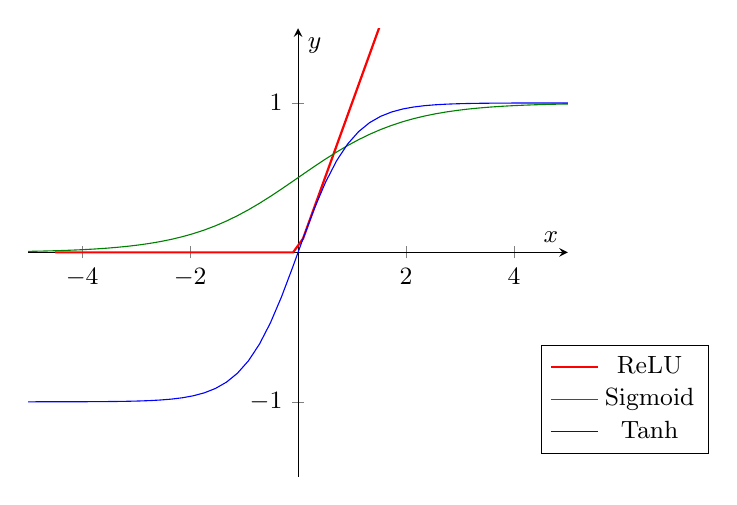
\begin{tikzpicture}
        \begin{axis}[
            axis lines = middle,
            xlabel = \(x\),
            ylabel = \(y\),
            xmin=-5.0,
            xmax=5.0,
            ymin=-1.5, 
            ymax=1.5,
            legend entries={ReLU,tanh,sigmoid},
            legend style={at={(0.95,0.05)},anchor=south west},
            %legend image post style={sharp plot,draw=red},
            cycle list name=color list,
            font=\small,
        ]
        % ReLU
        \addplot[color = red, thick, domain=-4.5:4.5, samples = 50] {max(0,x)};
        \addlegendentry{ReLU}
        % Sigmoid
        \addplot[color = green!50!black, samples=50] {1/(1+exp(-x))};
        \addlegendentry{Sigmoid}
    
        % tanh
        \addplot[color = blue, samples=50] {tanh(x)};
        \addlegendentry{Tanh}
        \end{axis}
    \end{tikzpicture}
    \caption{Activation Functions (ReLU, Sigmoid, Tanh) - Activation functions determine the output of a neuron in a neural network, and ReLU, Sigmoid, and Tanh are some commonly used activation functions that enable non-linear transformations of input data.}
    \label{fig:Activation Functions}
\end{figure}


\subsection{Hidden Layers}
Many issues can be solved by starting with a single hidden layer and producing acceptable results. Even the most complex functions can theoretically be modeled by an MLP with just one hidden layer. Deep networks, however, outperform shallow ones in terms of \textit{parameter efficiency} for complicated situations. Deep neural networks benefit from the fact that real-world data is frequently hierarchically structured as follows: The output layer and the highest hidden layers combine these intermediate structures to model high-level structures. Lower hidden layers model low-level structures, intermediate hidden layers combine these low-level structures to model intermediate-level structures, and the highest hidden layers model high-level structures like faces.

In conclusion, the neural network will function properly in many situations if you start with just one or two hidden layers. Increase the number of hidden layers for more complicated problems until the training set starts to become overfit. Large picture classification or speech recognition are two examples of extremely hard jobs that generally demand networks with dozens of layers and a huge amount of training data.

\subsection{Learning Rate and Optimizer}
There are more hyperparameters in an MLP than the number of neurons and hidden layers that can be changed. Some of the most important are listed below:
\paragraph{Learning rate} \mbox{} \\
\noindent The learning rate is the most important hyperparameter. The ideal learning rate is often equal to half the maximum learning rate.  Training the model for a few hundred iterations with a very low learning rate, like $10^{-5}$, and progressively raising it to a very high number, like $10$, is one method of determining a good learning rate. If you plot the loss as a function of the learning rate, you should notice that it first decreases.
However, after a while, the learning rate will become excessive, causing the loss to quickly increase again. The optimal learning rate will be slightly lower than the point at which the loss begins to increase.

\paragraph{Optimizer}\mbox{}\\
Equally important is selecting a better optimizer than just an odd mini-batch gradient descent. There are several optimizers that you can use to speed up the training but we are going to see just one, \textit{Adam}.
Adam -, which stands for \textit{adaptive moment estimation}, combines the concepts of momentum optimization and RMSProp: it tracks an exponentially decaying average of previous gradients, just like momentum optimization, and just like RMSProp, it tracks an exponentially decaying average of previously squared gradients. These are estimates of the gradients' mean and variance. The algorithm's name comes from the fact that the mean is sometimes referred to as the first instant and the variance as the second.
In other words, we can say the algorithm keeps track of two moving averages: the mean and the variance of the gradients; these moving averages are updated at each training step. This allows the algorithm to adapt to changes in the distribution of the gradients, which can be very beneficial for training deep neural networks:

\begin{equation}
    t = t + 1 
    \label{eq:1}
\end{equation}
\begin{equation}
    m_t = \beta_1 \cdot m_{t-1} + (1 - \beta_1) \cdot \nabla_{\theta} J(\theta) 
    \label{eq:2}
\end{equation}
\begin{equation}
    v_t = \beta_2 \cdot v_{t-1} + (1 - \beta_2) \cdot (\nabla_{\theta} J(\theta))^2 \label{eq:3}
\end{equation}
\begin{equation}
    \hat{m}_t = \frac{m_t}{1 - \beta_1^t}
    \label{eq:4}
\end{equation}
\begin{equation}
    \hat{v}_t = \frac{v_t}{1 - \beta_2^t}
    \label{eq:5}
\end{equation}
\begin{equation}
    \theta = \theta - \alpha \cdot \frac{\hat{m}_t}{\sqrt{\hat{v}_t} + \epsilon}
    \label{eq:6}
\end{equation}

where $\theta$ represents the parameters of the model, $\nabla_{\theta} J(\theta)$ is the gradient of the cost function J with respect to the parameters $\theta$, $\beta_1$ and $\beta_2$ are the decay rates of the moving averages, $\alpha$ is the learning rate, and $\epsilon is$ a small constant added to the denominator to prevent division by zero.

\hspace{1cm}

At each time step $t$, the mean $m_t$ and the variance $v_t$ of the gradients are updated using the equations \eqref{eq:2} and \eqref{eq:3}. Here, $m_{t-1}$ and $v_{t-1}$ represent the moving averages of the gradients and their squares from the previous time step. $\beta_1$ and $\ beta_2$ are hyperparameters that control the decay rate of the moving averages. They determine the amount of weight given to the past values of the gradients and their squares and the amount of weight given to the current gradient and its square.
After updating $m_t$ and $v_t$, the moving averages are corrected for bias using the equations \eqref{eq:4} and \eqref{eq:5}. The bias correction ensures that the moving averages are a better estimate of the true mean and variance of the gradients, especially at the start of the optimization process when $t$ is small.
Finally, the parameters $\theta$ are updated using the equation \eqref{eq:6}. Here, $\alpha$ is the learning rate, which determines the step size at which the parameters are updated. The term $\frac{\hat{m}_t}{\sqrt{\hat{v}_t} + \epsilon}$ is an approximation of the gradient of the cost function $J$ with respect to the parameters $\theta$. The addition of $\epsilon$ in the denominator is used to prevent division by zero.

This update rule balances the magnitude of the steps taken in the direction of the gradient with the magnitude of the gradient itself, allowing the optimization algorithm to make large steps in the directions with a high gradient and small steps in the directions with a low gradient. This makes the optimization process more efficient and helps the algorithm avoid getting stuck in local minima.
There are three variants of Adam: AdaMax, Nadam, and Adam W.

\subsection{Batch Normalization}
The danger of the vanishing/exploding gradients problems can be considerably reduced at the beginning of training by employing Glorot initialization in conjunction with ReLU, but this does not ensure that they won't reappear later on.
In a 2015 paper -, Sergey Ioffe and Christopher Szegedy suggested a method to solve these issues called \textit{batch normalization} (BN). The procedure includes inserting an operation into the model just before or after each hidden layer's activation function. The technique helps the model discover the ideal mean and scale for each input layer. In many circumstances, standardizing your training set is unnecessary if you include a BN layer as the initial layer of your neural network.

\hspace{1cm}

Let's say that we have a mini-batch of N examples, and the activations for a particular layer for one example is given by $X = [x_1, x_2, ..., x_d]$, where d is the number of neurons in the layer. The batch normalization algorithm consists of the following steps:

\begin{enumerate}
\item Calculate the mean and variance of the activations for the mini-batch:

\begin{equation}
\text{mean} = \frac{1}{N} \sum_{i=1}^{N} X_i
\end{equation}

\begin{equation}
\text{variance} = \frac{1}{N} \sum_{i=1}^{N} (X_i - \text{mean})^2
\end{equation}

\item Normalize the activations:

\begin{equation}
\hat{X} = \frac{X - \text{mean}}{\sqrt{\text{variance} + \epsilon}}
\end{equation}

where $\epsilon$ is a small constant added for numerical stability.

\item Scale and shift the normalized activations:

\begin{equation}
X_{\text{bn}} = \gamma \cdot \hat{X} + \beta
\end{equation}

where $\gamma$ and $\beta$ are learnable parameters.

\item Use the normalized and scaled activations as inputs to the next layer in the network.
\end{enumerate}

It is important to note that during training, the mean and variance of the activations are calculated on each mini-batch. During inference, the mean and variance are estimated using a running average that is updated during training. This allows the batch normalization layer to normalize the activations in a way that is consistent with the training data. In summary, the batch normalization algorithm normalizes the activations of a layer in a deep neural network by subtracting the mean and dividing by the standard deviation, scaling and shifting the result using learnable parameters, and using the normalized activations as inputs to the next layer in the network.

\hspace{1cm}

In conclusion, batch normalization is a widely used and effective technique for improving the training and performance of deep neural networks. It can help speed up training, prevent overfitting, and make the training process more robust to changes in the scale of the inputs and weights.

\subsection{Dropout}
Dropout, Figure \ref{fig:Dropout}, is one of the most popular regularization techniques for deep neural networks. It was proposed in a paper - by Geoffry Hinton et al. in 2012. 
It is a relatively straightforward algorithm: at each training step, each neuron (including input neurons but never output neurons) has a probability $p$ of being temporarily "dropped out," which means it will be completely ignored during this training phase but may be active during the next. This means that their activations are set to zero, and their incoming and outgoing connections are ignored. This has the effect of reducing the number of parameters in the network and making it more difficult for the network to memorize the training data. The dropout rate, also known as the hyperparameter p, is normally set between 10\% and 50\%; in recurrent neural networks, it is more likely to be between 20\% and 30\%. 

\begin{figure}[h!]
    \centering
    \begin{tikzpicture}[node/.style={circle, draw, thick}, scale = 0.85, transform shape]

      \foreach \y in {1,...,5}{
          \node[node] (i\y) at (0,\nodesep*\y) {};
          \node[node, right=\layersep of i\y] (h1\y) {};
          \node[node, right=\layersep of h1\y] (h2\y) {};
        }
    
      \node[node, right=\layersep of h22] (o1) {};
      \node[node, right=\layersep of h24] (o2) {};
    
      \foreach \source in {1,...,5}
      \foreach \dest in {1,...,5}{
          \path[-stealth, thick] (i\source) edge (h1\dest);
          \path[-stealth, thick] (h1\source) edge (h2\dest);
        }
      \foreach \source in {1,...,5}
      \foreach \dest in {1,2}
      \draw[-stealth, thick] (h2\source) -- (o\dest);
    
      \draw[-stealth, thick] (7.5,3*\nodesep) -- node[above,font=\Large\bfseries] {dropout} (9.5, 3*\nodesep);
    
      % Boundary
    
      \foreach \y in {1,...,5}
      \node[node, right=15em of h2\y] (di\y) {};
    
      \node[red,font=\huge] at (di1) {$\times$};
      \node[red,font=\huge] at (di3) {$\times$};
    
      \foreach \y in {1,...,5}
      \node[node, right=\layersep of di\y] (dh1\y) {};
    
      \node[red,font=\huge] at (dh11) {$\times$};
      \node[red,font=\huge] at (dh13) {$\times$};
      \node[red,font=\huge] at (dh14) {$\times$};
    
      \foreach \y in {1,...,5}
      \node[node, right=\layersep of dh1\y] (dh2\y) {};
    
      \node[red,font=\huge] at (dh22) {$\times$};
      \node[red,font=\huge] at (dh24) {$\times$};
    
      \node[node, right=\layersep of dh22] (do1) {};
      \node[node, right=\layersep of dh24] (do2) {};
    
      \foreach \source in {2,4,5}
      \foreach \dest in {2,5}
      \draw[-stealth, thick] (di\source) -- (dh1\dest);
    
      \foreach \source in {2,5}
      \foreach \dest in {1,3,5}
      \draw[-stealth, thick] (dh1\source) -- (dh2\dest);
    
      \foreach \source in {1,3,5}
      \foreach \dest in {1,2}
      \draw[-stealth, thick] (dh2\source) -- (do\dest);
    
    \end{tikzpicture}
    \caption{Dropout Scheme - A regularization technique used in neural networks to prevent overfitting by randomly dropping out some of the neurons in the network during training.}
    \label{fig:Dropout}
\end{figure}


For example, if the dropout rate is 0.5, then during each training iteration, on average, half of the units in the network will be dropped out. This results in a different, randomly perturbed network architecture at each training iteration, which helps prevent overfitting. The dropout rate can be tuned through experiments to find the optimal value for a given problem and network architecture. In general, a dropout rate of 0.5 is a good starting point, but the optimal value will depend on the specifics of the problem and the network architecture.